\section{Feature engineering}\label{sec:4}

\begin{disposition}
This is the core of the report. We will tell it as a story in stages, because each stage was motivated by what the previous one could not do. For every stage we state the idea, the physical or economic reason behind it, the measured effect (Figure~\ref{fig:4.1}) and our best explanation of \emph{why} it worked or did not.
\end{disposition}

% Final text:


\begin{figure}[H]
  \centering
  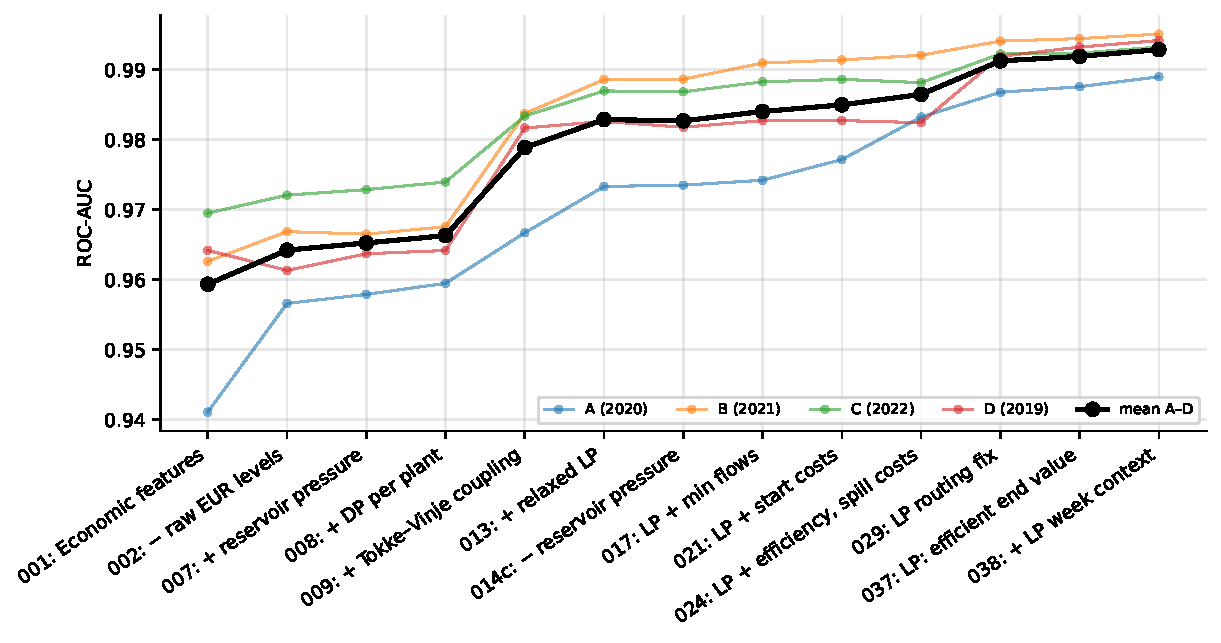
\includegraphics[width=\linewidth]{figures/fig_4_1.pdf}
  \caption{Validation AUC along the accepted changes}
  \label{fig:4.1}
\end{figure}

\subsection{Principles we followed}\label{sec:4.1}

\begin{disposition}
\begin{itemize}
\tightlist
\item
  \emph{Only use what SHOP knew.} Every feature is computed from the case's own inputs: prices, inflows and constraints inside the week, the volume at the start, and the water values at the start and at +7 days. Reservoir volumes after the start day are observed outcomes and would leak information, so they are never used. Neither is the optimiser's calculation time. One borderline case: two scarcity features use the mean price of the week \emph{after} the case. This is not label leakage, because the +7-day water value that SHOP received already reflects that price, but it is information from outside the case week.
\item
  \emph{Relative, not absolute, prices.} Because the price level changes by a factor of 20 between years (Figure~\ref{fig:2.5}), features are expressed relative to the week's price level (ranks, z-scores, differences divided by the level). A tree that learns ``on if price \textgreater{} 100 EUR'' in 2022 would fail in 2020 and in the test years.
\item
  \emph{Feature extraction over feature selection.} Most of our work is feature \emph{extraction} (building new features from physics). Feature \emph{selection} was done by group: a group was added only if it passed the acceptance rule, and from time to time we removed one group at a time (ablation) to check that it was still needed.
\end{itemize}
\end{disposition}

% Final text:


\subsection{Overview: the features we kept and the features we tried}\label{sec:4.overview}

% Final text:
Before going through the stages one by one, Tables~\ref{tab:4.groups} and~\ref{tab:4.tried} give an overview. The features are organised in \emph{feature groups}. A group is a set of features built from the same idea, for example ``how expensive is this hour compared with the rest of the week''. We added and removed whole groups rather than single features, for three reasons. First, the features in a group answer the same question in slightly different ways, so testing the group tests the idea itself. Second, the score varies by up to 0.0008 just from changing the random seed (Section~\ref{sec:3}); with up to 56 features, testing them one at a time would mean hundreds of comparisons, and some would look like improvements by pure luck. Third, a tree model is not harmed much by a few redundant features, because it simply does not split on a feature that adds nothing, so there was little to gain from removing single features.

Both final models, exp 038 (LightGBM) and exp 041 (XGBoost), use the same 12 groups with 56 features in total (Table~\ref{tab:4.groups}). The groups build on each other: the first eight describe the economics of each hour and the state of the reservoirs, the dynamic programme and the Tokke--Vinje coupling add the plants' schedules and how they depend on each other, the relaxed LP adds the physics of the whole watercourse (it is described as a predictor in Section~\ref{sec:5.lp}), and the LP week context gives each hour the LP's view of the rest of the week. Six features in raw EUR were built but removed from the model (Section~\ref{sec:4.3}). The full list of features with readable names is in Table~\ref{tab:A.1}.

\begin{table}[H]
  \centering\small
  \caption{The feature groups in the final models (exp 038 and 041)}
  \label{tab:4.groups}
  \begin{tabular}{>{\raggedright\arraybackslash}p{0.15\linewidth}r>{\raggedright\arraybackslash}p{0.32\linewidth}>{\raggedright\arraybackslash}p{0.35\linewidth}}
    \toprule
    \textbf{Group} & \textbf{Features} & \textbf{What it describes} & \textbf{Why we included it} \\
    \midrule
    Price shape & 4 & How expensive the hour is compared with the rest of the week (z-score, rank, price divided by the week's level, and the 24-hour average around the hour). & SHOP moves water to the most expensive hours of the week. Relative prices keep their meaning even though the price level changes by a factor of 20 between years. \\
    Calendar & 4 & Hour within the case, hour of day, and the day of year and weekday the case starts. & Hour within the case captures effects near the end of the week; hour of day the daily price and demand pattern; day of year the season (snowmelt gives high inflow in spring). \\
    Water value & 2 & The net water value relative to the week's price level, and how the water value changes over the week. & A rising water value means water is becoming more valuable, which is a reason to save it. \\
    Reservoirs & 3 & Fill of the reservoir above and below the plant on the start day, and the week's inflow. & A nearly full reservoir must release water, an empty one cannot, and a full reservoir below limits how much the plant can release. \\
    Unit & 3 & Unit ID, maximum output and start cost. & Lets one pooled model treat the 14 units differently. Large units and units with high start costs need a larger margin to be worth starting. \\
    Price vs water value & 4 & The margin: price minus the water value, in four versions (upstream only, net of the downstream value, and as a ratio). & This is the core of SHOP's decision: run when the water earns more now than it is worth if saved. The versions are scaled differently, and the trees use the one that splits best. \\
    Scarcity & 3 & The water value divided by the mean price at the start and end of the week, and next week's price level. & Expresses how scarce water is in a way that can be compared across years. Uses next week's mean price, which the +7-day water value already reflects. \\
    Week economics & 2 & Share of the week's hours with a positive margin, and the total positive margin. & Describes the week as a whole: if most hours are profitable, the unit will run a lot. \\
    Dynamic programme & 6 & For each plant, the most profitable on/off schedule with start costs: on or off, how many units, and the regret (how much is lost by doing the opposite). Solved with the YAML start cost and with 10 times that cost. & Adds start costs, which make units run in blocks instead of switching every hour. The regret acts as a confidence measure. Two cost levels because we did not know the scale SHOP uses. \\
    Tokke--Vinje coupling & 3 & The partner plant's schedule, regret and margin. & Vinje releases into the tiny Vinjevatn, which Tokke must empty, so the two plants run together. \\
    Relaxed LP & 5 & Production, units on, margin, hourly water value and reservoir fill from the LP of the whole watercourse. Water left at the end of the week is valued at the plants' best efficiency (Section~\ref{sec:4.lpweek}). & Our simplified copy of SHOP's own optimisation, including reservoir limits and the flow between all reservoirs (Section~\ref{sec:5.lp}). \\
    LP week context & 17 & Rolling 6~h and 24~h means and the week's mean, minimum and maximum of the LP's unit on and margin; the share of hours with a positive LP margin; Tokke's and Vinje's LP production and margin; and the start-cost regret computed on the LP margin. & Each row sees one hour, but whether a unit runs depends on the rest of the week. These features tell the hour whether it is one of the few good hours or part of a week where the unit runs all the time. \\
    \midrule
    \textbf{Total} & \textbf{56} & & \\
    \bottomrule
  \end{tabular}
\end{table}

Table~\ref{tab:4.tried} lists every group we tried, why we expected it to help, and why it was kept or dropped. The gain is the change in mean AUC over folds A--D compared with the model it was added to. A group was kept only if it passed the acceptance rule (Section~\ref{sec:3}): a gain of at least 0.001, at least three of four folds not worse, and no fold worse by more than 0.002.

\begin{table}[H]
  \centering\small
  \caption{Every feature group we tried, why, and the decision}
  \label{tab:4.tried}
  \begin{tabular}{>{\raggedright\arraybackslash}p{0.14\linewidth}>{\raggedright\arraybackslash}p{0.08\linewidth}>{\raggedright\arraybackslash}p{0.29\linewidth}>{\raggedright\arraybackslash}p{0.09\linewidth}>{\raggedright\arraybackslash}p{0.26\linewidth}}
    \toprule
    \textbf{Group (features)} & \textbf{Exp} & \textbf{Why we tried it} & \textbf{Gain} & \textbf{Decision and why} \\
    \midrule
    Raw EUR levels (6) & 002 & Part of the first baseline: the price and water values in EUR. & +0.0049 when removed & \textbf{Removed.} The trees learned EUR thresholds that only hold in one price regime (Section~\ref{sec:4.3}). \\
    Margin context (15) & 005 & Units run in blocks because of start costs, so the margin in the hours around $t$ might matter, not only at $t$. & +0.0007 & \textbf{Dropped.} Within seed noise. The trees can already combine the margin with the price shape, so this only re-expresses existing information. \\
    Profitable blocks (5) & 006 & A long run of profitable hours justifies paying a start cost; a short one does not. & +0.0004 & \textbf{Dropped.} Same explanation as margin context. \\
    Reservoir pressure (2) & 007 & A nearly full reservoir with high inflow must release water whatever the price. & +0.0010 & \textbf{Kept, later removed} (exp 014c, $-0.0002$ without it): the LP already knows the reservoir limits. \\
    Dynamic programme (6) & 008 & Adds start costs and realistic on/off blocks per plant. & +0.0011 & \textbf{Kept.} Still needed with the LP ($-0.0011$ without it, exp 014a). \\
    Tokke--Vinje coupling (3) & 009 & Vinje and Tokke are linked by a tiny reservoir and run together. & +0.0126 & \textbf{Kept.} The largest gain before the LP; $-0.0071$ without it (exp 014b). \\
    Cascade (2) & 011 & The same idea as the coupling, for every plant fed by another plant. & +0.0008 & \textbf{Dropped.} Below the threshold. Hogga (fed by Tokke via Bandak) improved by 0.02--0.04 on all folds, but Lio and Kjela were mixed. The LP, added next, models all these connections anyway. \\
    Relaxed LP (5) & 013 & A simplified copy of SHOP's optimisation over the whole watercourse. & +0.0040 & \textbf{Kept}, and improved in four steps (017, 021, 024, 029: +0.0085 together; Section~\ref{sec:4.9}), then given a better end-of-week value (037, +0.0007; Section~\ref{sec:4.lpweek}). \\
    Real storage lake (3) & 019 & Haukeli's own reservoir data is a constant placeholder, so we used the lake above it instead. & +0.0001 & \textbf{Dropped.} The LP already models the lake above. \\
    Water budget (7) & 025 & How many full-power hours of water the plant must and can use this week. & +0.0010 without LP, +0.0001 with LP & \textbf{Dropped.} It helps only without the LP, which shows that the LP already computes the same information. \\
    Forward margin (6) & 026 & What the rest of the week still offers, which decides whether to use water now or later. & +0.0001 without and with LP & \textbf{Dropped.} No gain even without the LP: the price rank and the DP schedule already describe the rest of the week. \\
    Head (2) & 027 & The height drop sets how much power each m$^3$ of water gives. & 0.0000 without LP, $-0.0002$ with LP & \textbf{Dropped.} No gain even without the LP. Likely reason: the head follows the reservoir fill, which the model already has. \\
    Extra LP outputs (3) & 031 & More detail from the LP for the weakest units (Vinje G2/G3, Kjela). & $\pm 0.0001$ & \textbf{Dropped.} The trees could already recover this from the other LP and DP features. \\
    LP week context (17) & 038 & Whether a unit runs in one hour depends on the rest of the week, and the LP's weekly profile already includes the reservoir limits and the coupling. & +0.0016 vs 029 (with 037) & \textbf{Kept.} All four folds improve; twice the seed noise (Section~\ref{sec:4.lpweek}). \\
    \bottomrule
  \end{tabular}
\end{table}

\subsection{Stage 1: economic features (exp 001, mean AUC 0.9593)}\label{sec:4.2}

\begin{disposition}
Our first harness model used price shape (rank and z-score within the week), calendar, the price − water value margins, scarcity coefficients (how full the reservoir is, according to the water value), reservoir fill and inflow, and unit properties. We will explain each family in one or two sentences using the feature table.
\end{disposition}

% Final text:


\subsection{Removing raw EUR levels (exp 002, +0.005; 2020 +0.016)}\label{sec:4.3}

\begin{disposition}
Removing the six features in raw EUR (the price itself, the week's mean price and the raw water values) \emph{improved} the score, most clearly for 2020 when prices were extremely low. Explanation: the trees had learned thresholds in EUR that only hold in the price regime they were trained on. This is a feature-selection result worth highlighting.
\end{disposition}

% Final text:


\subsection{Rearranging the margin does not help (exps 005, 006)}\label{sec:4.4}

\begin{disposition}
Margins in neighbouring hours, rolling means and the length of profitable blocks gave nothing beyond noise. Explanation: a tree model can already combine the existing margin and price-shape features. \emph{Lesson we will state explicitly:} gains come from \emph{new information}, not from re-expressing existing information. \emph{Correction found later (Section~\ref{sec:4.lpweek}):} the same kind of summary over the week \emph{did} help when it was computed from the LP's outputs instead of the simple margin. So the lesson must be stated more carefully: rearranging a weak signal does not help, but summarising a strong one can.
\end{disposition}

% Final text:


\subsection{Reservoir pressure (exp 007, kept; later removed in exp 014c)}\label{sec:4.5}

\begin{disposition}
Week inflow divided by the free space in the reservoir: a nearly full reservoir with high inflow must produce or spill water, whatever the price. It helped 2019, but once the LP was added it became redundant (the LP knows the reservoir limits) and the ablation removed it. Good example of a feature that was useful at one stage and redundant at the next.
\end{disposition}

% Final text:


\subsection{A dynamic programme per plant (exp 008, +0.001, all folds up)}\label{sec:4.6}

\begin{disposition}
We will explain in plain words: for each plant, we search all on/off paths over the week and pick the one with the highest profit (price − water value, times production) minus start costs. This is cheap (milliseconds per case) and gives a schedule that already has realistic blocks instead of hour-by-hour switching. The most useful output was the \emph{regret}: how much profit would be lost by doing the opposite in that hour. It acts as a confidence measure. Why the gain was modest: the DP treats each plant separately and ignores reservoir limits.
\end{disposition}

% Final text:


\subsection{Tokke–Vinje coupling (exp 009, +0.013, the largest single jump before the LP)}\label{sec:4.7}

\begin{disposition}
Each Tokke unit gets Vinje's DP schedule and margin, and the other way round. Explanation: Vinje releases into the tiny Vinjevatn, which Tokke must empty, so when Vinje G1 runs, Tokke G1 runs 99.5\% of the time (otherwise 37\%). The partner features are weak alone but strong together with the unit's own features, which is exactly the kind of interaction trees are good at. Tokke G2--G4 improved by 0.02--0.08.
\end{disposition}

% Final text:


\subsection{The relaxed LP of the whole watercourse (exp 013, +0.004; the most important feature)}\label{sec:4.8}

% Final text:
The relaxed LP is described as a predictor in Section~\ref{sec:5.lp}. Here we look at it as a feature group. Adding its five outputs (production, units on, margin, hourly water value and fill) to exp 009 raised the mean AUC from 0.9789 to 0.9829, with all four folds improving, and the LP features became the most important in the model (Section~\ref{sec:7}).

\emph{Why it works so well.} The labels \emph{are} the solution of almost the same optimisation problem. The features before the LP each describe one part of the decision: the margin describes the economics of one hour, the fill describes one reservoir, the DP describes one plant without reservoir limits. The LP combines all of these in one consistent solution for the whole watercourse and the whole week. The learned model then no longer has to reconstruct SHOP's decision from the parts; it only has to learn where the simplified LP differs from SHOP, for example that the LP tends to commit too many units.

\emph{Why the earlier groups were still needed.} The ablations showed that the DP ($-0.0011$ without it) and the Tokke--Vinje coupling ($-0.0071$) still helped next to the LP, while reservoir pressure did not (Table~\ref{tab:4.tried}). The first LP version had no start costs and no unit commitment, so the DP's on/off blocks and the coupling's partner schedules added information it did not have. Reservoir pressure did not, because the LP already knows the reservoir limits.

\emph{A failure that taught us something.} Water left at the end of the week will later run through every plant below it on its way to the sea, so its value depends on how much power it can still produce. We tried two ways of pricing that power. In the ``sea'' valuation, all the power the water could produce down to the sea was priced at the water value of the reservoir it is left in. This made the LP much worse: on a sample of the training weeks, the AUC of its units on fell from 0.889 to 0.726 and of its margin from 0.929 to 0.789. In the ``path'' valuation, which we use, the power from each plant on the way is priced at the water value of the reservoir that feeds that plant. Our explanation is that the synthetic water values of neighbouring reservoirs are not consistent with each other, so pricing a whole chain of plants with one reservoir's water value gives the wrong incentives, while the path valuation lets every plant compare the price with its own upstream water value, which is what the labels follow (Section~\ref{sec:2}).

\subsection{Making the LP more like SHOP (exps 017, 021, 024, 029; 0.9840 → 0.9912)}\label{sec:4.9}

\begin{disposition}
We improved the LP step by step and measured each step separately:

\begin{itemize}
\tightlist
\item
  \emph{Minimum river flows (017):} Lio improved by 0.02--0.07, because a minimum-flow requirement on its river forces it to run.
\item
  \emph{Relaxed unit commitment (021):} start/stop costs and minimum production inside the LP, which improves timing.
\item
  \emph{Efficiency curves and SHOP's spill costs (024):} mostly helped 2020, when water values were near zero and the old LP could ``dump'' water for free.
\item
  \emph{The routing bug fix (029, +0.0047, all folds up):} this is our case study, explained in plain words. The LP picked the \emph{first} river leaving each reservoir. For Hyljelihyl that is a bypass that skips the Vinje plant, while the topology file marks another river (via Totak to Vinje) as the main one. Water left in Hyljelihyl, and in every lake above it, was therefore valued too low, which made running Kjela look too attractive and distorted the water prices along the Totak--Vinje--Tokke chain. Fixing it improved Haukeli from 0.923 to 0.974 and Kjela from 0.977 to 0.989. \emph{Lesson:} checking that the model's physics is right was worth more than any tuning.
\item
  We will also mention LP variants that were tested and dropped (head iterations, integer units, alternative valuations), with one line each.
\end{itemize}
\end{disposition}

% Final text:


\subsection{Efficient end-of-week value and the LP over the whole week (exps 037, 038; 0.9912 → 0.9929)}\label{sec:4.lpweek}

The last round of feature work made two changes on top of exp 029. Both final models use them.

\emph{Valuing leftover water at the best efficiency (exp 037, +0.0007, all four folds up).} The LP turns the water left at the end of the week into money through the end-of-week water value, which is in EUR/MWh, so it has to convert cubic metres of water into MWh. Until then it used each plant's average efficiency at full load. Exp 037 uses the efficiency of the first and most efficient production segment instead. This is closer to how the water will actually be used later, and it values saved water higher, so the LP holds back more water. Only the value of the leftover water changes; production inside the week is modelled as before. On a sample of the training weeks (every sixth case), the AUC of the LP's units on alone rose from 0.9447 to 0.9597, and of the LP margin alone from 0.9739 to 0.9770. The gain in the learned model (+0.0007) was below the acceptance threshold on its own.

\emph{The LP over the whole week (exp 038, +0.0016 over 029, all four folds up).} Each training row describes one unit in one hour, but whether a unit runs in that hour depends on the rest of the week: a start cost is only worth paying if the unit then runs for a while. The 17 features of the LP week context (Table~\ref{tab:4.groups}) give the hour that context, all computed from the LP's outputs. They include rolling 6~h and 24~h means of the LP's units on and margin, the week's mean, minimum and maximum of both, the share of hours with a positive LP margin, and Tokke's and Vinje's LP production and margin for every unit. The last feature is a start-cost regret: the dynamic programme of Section~\ref{sec:4.6}, run on the LP margin instead of on the simple price minus water value margin.

\emph{Why this worked when the rolling margins of exp 005 did not.} The LP margin already includes the reservoir limits, the coupling between plants and the hourly water values, so its profile over the week carries much more information than the profile of the simple margin. Our best explanation is that this weekly view (is this hour one of the few good ones, or is the unit on all week?) is hard for a tree to rebuild from the values of a single hour.

\emph{The gain is not specific to LightGBM.} The XGBoost twin, exp 041, uses the same 56 features with the settings of exp 030. It gains +0.0017 over exp 030, and all four folds improve. The gain therefore comes from the features, not from one model type.

\emph{Protocol, stated openly.} Exp 037 failed the acceptance rule on its own but was kept and combined with the week context in exp 038, and the week context was never tested without 037. The combined gain of exp 038 (+0.0016) is twice the seed noise (0.0008), and every fold improves. A larger fit on the same features (exp 039: 60\% of the rows and 2200 trees) gave only +0.0002 more, below the noise, so it was not selected (Section~\ref{sec:6}).

\emph{Tried and dropped.} Sixteen production segments in the LP instead of four gave no clear gain on the LP sanity check. A separate model for each unit's share of hours on in the week added +0.00005. Smoothing the predicted probabilities over the hours (median filter, or smoothing of probabilities or logits) gave no gain.

\subsection{What did not help once the LP was in (exps 019, 025–027, 031)}\label{sec:4.10}

\begin{disposition}
A water budget, forward-looking margins, head proxies, the real storage lake behind Haukeli, an unclipped LP units-on gap and the joint fill of lakes joined by tunnels all gave at most ± 0.0002 on top of the LP (Table~\ref{tab:4.tried}). For the water budget, the storage lake and the extra LP outputs, the explanation is that the LP already computes this information; the water budget \emph{did} help the model without the LP (+0.001), which supports that explanation. Forward margins and head proxies did not help even without the LP, so for them the information was already in the earlier features (price rank and DP schedule, and reservoir fill).
\end{disposition}

% Final text:


\subsection{Summary of feature selection}\label{sec:4.11}

\begin{disposition}
The full experiment log (Table~\ref{tab:B.1} in Appendix~\ref{sec:B}) shows every change, its effect and the decision. The ablation (014a--c) showed that the DP (−0.0011 without it) and the coupling (−0.0071) are still needed next to the LP. Some redundant features remain (e.g.~two versions of the net margin) because tree models tolerate them and removing them did not change the score. Both final models, exp 038 (LightGBM) and exp 041 (XGBoost), use the same 56 features in 12 groups (Table~\ref{tab:A.1}); along the accepted changes the mean AUC rose from 0.9593 (exp 001) to 0.9929 (exp 038, Figure~\ref{fig:4.1}). Figure~\ref{fig:7.1} shows how much each feature family contributes to the LightGBM model.
\end{disposition}

% Final text:
